\documentclass[12pt]{article}
\usepackage[table]{xcolor}
\usepackage[shortlabels]{enumitem}
\usepackage{tabularx,xltabular}
\usepackage{graphicx}
\usepackage{hyperref}
\usepackage{verbatim}
\usepackage{geometry}
\usepackage{ulem}
\usepackage[official]{eurosym}
\usepackage{tikz}
\usetikzlibrary{arrows,backgrounds,calc,decorations.markings,patterns,3d,positioning,fit,angles, quotes}
\usepackage{pgfplots}
\pgfplotsset{compat = newest}
\usetikzlibrary{fit}
\newcommand\addvmargin[1]{
\usetikzlibrary{arrows}
\node[fit=(current bounding box),inner ysep=#1,inner xsep=0]{};}
\usepackage{cancel}
\usepackage{fontspec}
\usepackage{array}  
\geometry{a4paper, top=2cm, left=2cm, right=2cm, bottom=2cm, headsep=1cm}
\usepackage{tabu}
\usepackage{pst-node}
\usepackage{colortbl}
\usepackage{array}
\usepackage{german}
\setlength\parindent{0pt}
\newcolumntype{?}{!{\vrule width 1pt}}
\usepackage{makecell}
\renewcommand{\arraystretch}{2.5}
\usepackage{pbox}
\usepackage{amssymb}
\usepackage{amsmath}
\usepackage{booktabs}
\newcolumntype{L}[1]{>{\raggedright\let\newline\\\arraybackslash\hspace{0pt}}m{#1}}
\newcolumntype{C}[1]{>{\centering\let\newline\\\arraybackslash\hspace{0pt}}m{#1}}
\newcolumntype{R}[1]{>{\raggedleft\let\newline\\\arraybackslash\hspace{0pt}}m{#1}}
\begin{document}
\rightline{Datum: 08.12.2023}
\centerline{{\Large Üben für die Arbeit}} 
\vspace{1cm}
\noindent \\


\begin{xltabular}{\textwidth}{|C{0.75cm}|X|C{0.75cm}|X|}
\arrayrulecolor{black}\hline
a)&\pbox{5cm}{Wieviel Prozent sind schraffiert? \\
\tikzstyle{background grid}=[draw, black!15,step=.5cm]
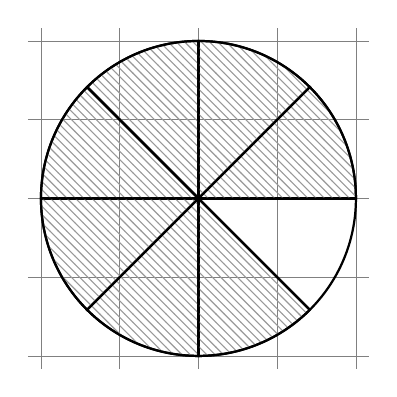
\begin{tikzpicture}[show background grid]
\pgfmathsetmacro{\R}{2}   
\draw[thick] (0,0) circle (\R); 
\draw[thick] (0,0) -- (90.0:\R);
\draw[thick] (0,0) -- (135.0:\R);
\draw[thick] (0,0) -- (180.0:\R);
\draw[thick] (0,0) -- (225.0:\R);
\draw[thick] (0,0) -- (270.0:\R);
\draw[thick] (0,0) -- (315.0:\R);
\draw[thick] (0,0) -- (360.0:\R);
\draw[thick] (0,0) -- (405.0:\R);
\draw[thick,pattern=north west lines, pattern color=black!40] (0,0) -- (360.0:\R) arc (360.0:405.0:\R) -- (0,0);
\draw[thick,pattern=north west lines, pattern color=black!40] (0,0) -- (225.0:\R) arc (225.0:270.0:\R) -- (0,0);
\draw[thick,pattern=north west lines, pattern color=black!40] (0,0) -- (90.0:\R) arc (90.0:135.0:\R) -- (0,0);
\draw[thick,pattern=north west lines, pattern color=black!40] (0,0) -- (270.0:\R) arc (270.0:315.0:\R) -- (0,0);
\draw[thick,pattern=north west lines, pattern color=black!40] (0,0) -- (135.0:\R) arc (135.0:180.0:\R) -- (0,0);
\draw[thick,pattern=north west lines, pattern color=black!40] (0,0) -- (405.0:\R) arc (405.0:450.0:\R) -- (0,0);
\draw[thick,pattern=north west lines, pattern color=black!40] (0,0) -- (180.0:\R) arc (180.0:225.0:\R) -- (0,0);
\end{tikzpicture}
}
&
b)&\pbox{5cm}{Wieviel Prozent sind schraffiert? \\
\tikzstyle{background grid}=[draw, black!15,step=.5cm]
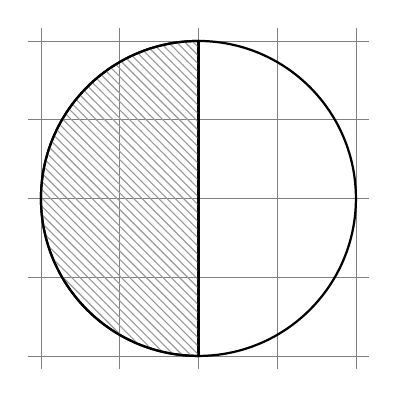
\begin{tikzpicture}[show background grid]
\pgfmathsetmacro{\R}{2}   
\draw[thick] (0,0) circle (\R); 
\draw[thick] (0,0) -- (90.0:\R);
\draw[thick] (0,0) -- (270.0:\R);
\draw[thick,pattern=north west lines, pattern color=black!40] (0,0) -- (90.0:\R) arc (90.0:270.0:\R) -- (0,0);
\end{tikzpicture}
}
\\\hline
c)&\pbox{5cm}{Wieviel Prozent sind schraffiert? \\
\tikzstyle{background grid}=[draw, black!15,step=.5cm]
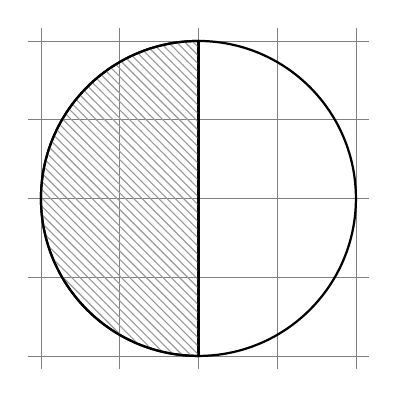
\begin{tikzpicture}[show background grid]
\pgfmathsetmacro{\R}{2}   
\draw[thick] (0,0) circle (\R); 
\draw[thick] (0,0) -- (90.0:\R);
\draw[thick] (0,0) -- (270.0:\R);
\draw[thick,pattern=north west lines, pattern color=black!40] (0,0) -- (90.0:\R) arc (90.0:270.0:\R) -- (0,0);
\end{tikzpicture}
}
&
d)&\pbox{5cm}{Wieviel Prozent sind schraffiert?\\
\tikzstyle{background grid}=[draw, black!15,step=.5cm]
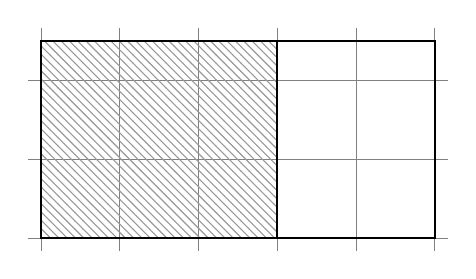
\begin{tikzpicture}[show background grid]
\pgfmathsetmacro{\laenge}{5}  
\pgfmathsetmacro{\hoehe}{\laenge/2}  
\pgfmathsetmacro{\percent}{60/100}  
\draw[thick] (0,0) rectangle ++ (\laenge,\hoehe);
\draw[thick,pattern=north west lines, pattern color=black!40] (0,0) rectangle ++ (\laenge*\percent,\hoehe);
\end{tikzpicture}
}
\\\hline
e)&\pbox{5cm}{Wieviel Prozent sind schraffiert?\\
\tikzstyle{background grid}=[draw, black!15,step=.5cm]
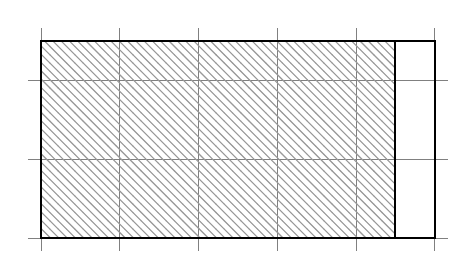
\begin{tikzpicture}[show background grid]
\pgfmathsetmacro{\laenge}{5}  
\pgfmathsetmacro{\hoehe}{\laenge/2}  
\pgfmathsetmacro{\percent}{90/100}  
\draw[thick] (0,0) rectangle ++ (\laenge,\hoehe);
\draw[thick,pattern=north west lines, pattern color=black!40] (0,0) rectangle ++ (\laenge*\percent,\hoehe);
\end{tikzpicture}
}
&
f)&\pbox{5cm}{Wieviel Prozent sind schraffiert?\\
\tikzstyle{background grid}=[draw, black!15,step=.5cm]
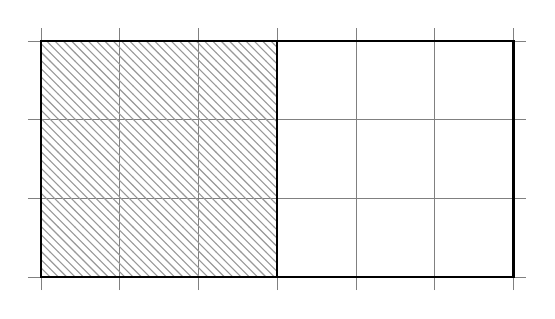
\begin{tikzpicture}[show background grid]
\pgfmathsetmacro{\laenge}{6}  
\pgfmathsetmacro{\hoehe}{\laenge/2}  
\pgfmathsetmacro{\percent}{50/100}  
\draw[thick] (0,0) rectangle ++ (\laenge,\hoehe);
\draw[thick,pattern=north west lines, pattern color=black!40] (0,0) rectangle ++ (\laenge*\percent,\hoehe);
\end{tikzpicture}
}
\\\hline
g)&Grundwert~1.000~kg;  Prozentsatz~2~\%
&
h)&Grundwert~400~kg;  Prozentsatz~5~\%
\\\hline
i)&Grundwert~400~km;  Prozentwert~40~km
&
j)&Grundwert~1.000~Schülerinnen;  Prozentwert~20~Schülerinnen
\\\hline
k)&Prozentwert~16~km;  Prozentsatz~4~\%
&
l)&Prozentwert~20~g;  Prozentsatz~10~\%
\\\hline
m)&Kapital~4.000~€;  Zinssatz~6~\%
&
n)&Kapital~2.750~€;  Zinssatz~4~\%
\\\hline
o)&Kapital~10.840~€;  Zinsen~271~€
&
p)&Kapital~11.875~€;  Zinsen~190~€
\\\hline
q)&Zinsen~200~€;  Zinssatz~2~\%
&
r)&Zinsen~130~€;  Zinssatz~5,2~\%
\\\hline
s)&Kapital 11.000 €;  Zinssatz 1  \%
&
t)&Kapital 10.500 €;  Zinsen 105  €
\\\hline
u)&Berechne die Monatszinsen für 2 Monate und $K=5.750~€$ bei $p~\%=4~\%$.
&
v)&Berechne die Monatszinsen für 7 Monate und $K=14.000~€$ bei $p~\%=2~\%$.
\\\hline
w)&Berechne das ersparte Geld nach 2 Jahren für K=4.280 € und p\%=2,5 \%
&
x)&Berechne das ersparte Geld nach 2 Jahren für K=13.950 € und p\%=2 \%
\\\hline
\end{xltabular}
\vspace{0.5cm}
\newpage
\rightline{Datum: 08.12.2023}
\centerline{{\large Lösungen Üben für die Arbeit}} 
\vspace{0.5cm}

\begin{xltabular}{\textwidth}{|C{0.75cm}|X|C{0.75cm}|X|}
\arrayrulecolor{black}\hline
a)&$$\frac{7}{8}=0,88=87,5\%$$
&
b)&$$\frac{1}{2}=0,5=50\%$$
\\\hline
c)&$$\frac{1}{2}=0,5=50\%$$
&
d)&\pbox{5cm}{
\tikzstyle{background grid}=[draw, black!15,step=.5cm]
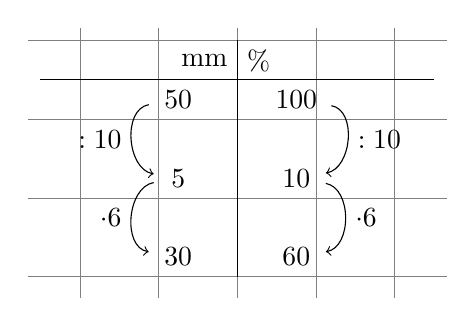
\begin{tikzpicture}[show background grid]
\draw[black] (0cm,0cm) -- (0cm,-3cm); 
\draw[black] (-2.5 cm,-0.5cm) -- (2.5cm,-0.5cm); 
\node[left] at (0 cm,-0.25cm) {mm};
\node[right] at (0 cm,-0.255cm) {\%};
\node[circle] (1) at (-0.75 cm,-0.75cm) {50};
\node[circle] (2) at (-0.75 cm,-1.75cm) {5};
\node[circle] (3) at (-0.75 cm,-2.75cm) {30};
\node[circle] (4) at (0.75 cm,-0.75cm) {100};
\node[circle] (5) at (0.75 cm,-1.75cm) {10};
\node[circle] (6) at (0.75 cm,-2.75cm) {60};
\draw[->] (1) to [out=190,in=170] node[left] {$:10$}  (2) ;
\draw[->] (2) to [out=190,in=170] node[left] {$\cdot 6$}  (3) ;
\draw[->] (4) to [out=350,in=10] node[right] {$:10$}  (5) ;
\draw[->] (5) to [out=350,in=10] node[right] {$\cdot6$}  (6) ;
\end{tikzpicture}
\newline
Oder: \newline
Gesamtlänge: 50\,mm, Länge der Schraffur: 30\,mm. Das bedeutet: \newline
$\frac{30}{50}=0,6=60\%$
}
\\\hline
e)&\pbox{5cm}{
\tikzstyle{background grid}=[draw, black!15,step=.5cm]
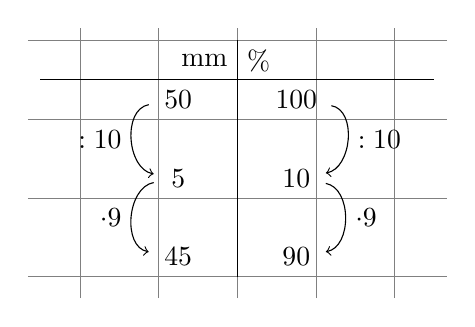
\begin{tikzpicture}[show background grid]
\draw[black] (0cm,0cm) -- (0cm,-3cm); 
\draw[black] (-2.5 cm,-0.5cm) -- (2.5cm,-0.5cm); 
\node[left] at (0 cm,-0.25cm) {mm};
\node[right] at (0 cm,-0.255cm) {\%};
\node[circle] (1) at (-0.75 cm,-0.75cm) {50};
\node[circle] (2) at (-0.75 cm,-1.75cm) {5};
\node[circle] (3) at (-0.75 cm,-2.75cm) {45};
\node[circle] (4) at (0.75 cm,-0.75cm) {100};
\node[circle] (5) at (0.75 cm,-1.75cm) {10};
\node[circle] (6) at (0.75 cm,-2.75cm) {90};
\draw[->] (1) to [out=190,in=170] node[left] {$:10$}  (2) ;
\draw[->] (2) to [out=190,in=170] node[left] {$\cdot 9$}  (3) ;
\draw[->] (4) to [out=350,in=10] node[right] {$:10$}  (5) ;
\draw[->] (5) to [out=350,in=10] node[right] {$\cdot9$}  (6) ;
\end{tikzpicture}
\newline
Oder: \newline
Gesamtlänge: 50\,mm, Länge der Schraffur: 45\,mm. Das bedeutet: \newline
$\frac{45}{50}=0,9=90\%$
}
&
f)&\pbox{5cm}{
\tikzstyle{background grid}=[draw, black!15,step=.5cm]
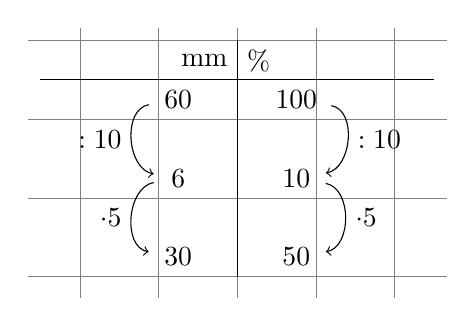
\begin{tikzpicture}[show background grid]
\draw[black] (0cm,0cm) -- (0cm,-3cm); 
\draw[black] (-2.5 cm,-0.5cm) -- (2.5cm,-0.5cm); 
\node[left] at (0 cm,-0.25cm) {mm};
\node[right] at (0 cm,-0.255cm) {\%};
\node[circle] (1) at (-0.75 cm,-0.75cm) {60};
\node[circle] (2) at (-0.75 cm,-1.75cm) {6};
\node[circle] (3) at (-0.75 cm,-2.75cm) {30};
\node[circle] (4) at (0.75 cm,-0.75cm) {100};
\node[circle] (5) at (0.75 cm,-1.75cm) {10};
\node[circle] (6) at (0.75 cm,-2.75cm) {50};
\draw[->] (1) to [out=190,in=170] node[left] {$:10$}  (2) ;
\draw[->] (2) to [out=190,in=170] node[left] {$\cdot 5$}  (3) ;
\draw[->] (4) to [out=350,in=10] node[right] {$:10$}  (5) ;
\draw[->] (5) to [out=350,in=10] node[right] {$\cdot5$}  (6) ;
\end{tikzpicture}
\newline
Oder: \newline
Gesamtlänge: 60\,mm, Länge der Schraffur: 30\,mm. Das bedeutet: \newline
$\frac{30}{60}=0,5=50\%$
}
\\\hline
g)&
\begingroup\setlength{\jot}{0.02cm}
\tikzstyle{background grid}=[draw, black!15,step=.5cm]
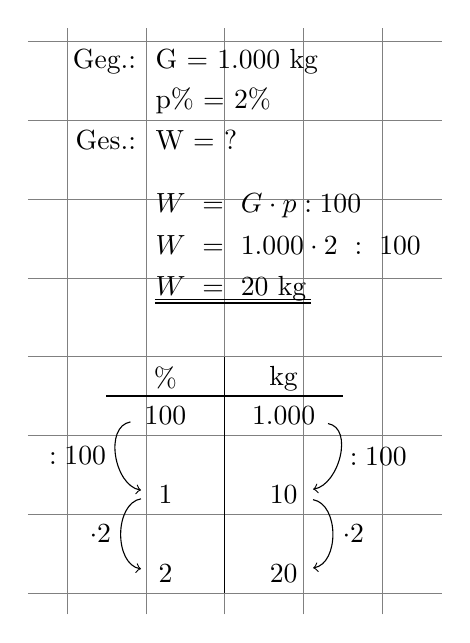
\begin{tikzpicture}[show background grid]
\node[left] at (0,-0.25) {Geg.: };
\node[right] at (0,-0.25) {G = 1.000 kg};
\node[right] at (0,-0.75) {p\% = 2\%};
\node[left] at (0,-1.-0.25) {Ges.: };
\node[right] at (0,-1.-0.25) {W  = ? };
\node[below right] at (0,-1.75) {
$\begin{aligned}
W\ &=\ G\cdot p : 100 \\
W\ &=\ 1.000\cdot 2\ :\ 100 \\
\makebox[0pt][l]{\uuline{\phantom{W\%\ =\ 20\ \mbox{kg}}}}
W\ &=\ 20\ \mbox{kg}
\end{aligned}$};

\draw[black] (1cm,-4cm) -- (1cm,-7cm); 
\draw[black] (-0.5 cm,-4.5cm) -- (2.5cm,-4.5cm); 
\node[below] at (0.25 cm,-4cm) {\%};
\node[below] at  (1.75 cm,-4cm) {kg};
\node[circle] (1) at (0.25 cm,-4.75cm) {100};
\node[circle] (2) at (0.25 cm,-5.75cm) {1};
\node[circle] (3) at (0.25 cm,-6.75cm) {2};
\node[circle] (4) at (1.75 cm,-4.75cm) {1.000};
\node[circle] (5) at (1.75 cm,-5.75cm) {10};
\node[circle] (6) at (1.75 cm,-6.75cm) {20};
\draw[->] (1) to [out=190,in=170] node[left] {$:100$}  (2) ;
\draw[->] (2) to [out=190,in=170] node[left] {$\cdot 2$}  (3) ;
\draw[->] (4) to [out=350,in=10] node[right] {$:100$}  (5) ;
\draw[->] (5) to [out=350,in=10] node[right] {$\cdot2$}  (6) ;
\end{tikzpicture}
\endgroup
&
h)&
\begingroup\setlength{\jot}{0.02cm}
\tikzstyle{background grid}=[draw, black!15,step=.5cm]
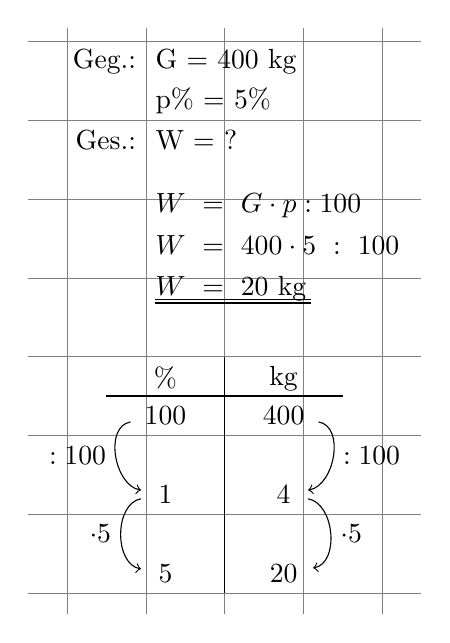
\begin{tikzpicture}[show background grid]
\node[left] at (0,-0.25) {Geg.: };
\node[right] at (0,-0.25) {G = 400 kg};
\node[right] at (0,-0.75) {p\% = 5\%};
\node[left] at (0,-1.-0.25) {Ges.: };
\node[right] at (0,-1.-0.25) {W  = ? };
\node[below right] at (0,-1.75) {
$\begin{aligned}
W\ &=\ G\cdot p : 100 \\
W\ &=\ 400\cdot 5\ :\ 100 \\
\makebox[0pt][l]{\uuline{\phantom{W\%\ =\ 20\ \mbox{kg}}}}
W\ &=\ 20\ \mbox{kg}
\end{aligned}$};

\draw[black] (1cm,-4cm) -- (1cm,-7cm); 
\draw[black] (-0.5 cm,-4.5cm) -- (2.5cm,-4.5cm); 
\node[below] at (0.25 cm,-4cm) {\%};
\node[below] at  (1.75 cm,-4cm) {kg};
\node[circle] (1) at (0.25 cm,-4.75cm) {100};
\node[circle] (2) at (0.25 cm,-5.75cm) {1};
\node[circle] (3) at (0.25 cm,-6.75cm) {5};
\node[circle] (4) at (1.75 cm,-4.75cm) {400};
\node[circle] (5) at (1.75 cm,-5.75cm) {4};
\node[circle] (6) at (1.75 cm,-6.75cm) {20};
\draw[->] (1) to [out=190,in=170] node[left] {$:100$}  (2) ;
\draw[->] (2) to [out=190,in=170] node[left] {$\cdot 5$}  (3) ;
\draw[->] (4) to [out=350,in=10] node[right] {$:100$}  (5) ;
\draw[->] (5) to [out=350,in=10] node[right] {$\cdot5$}  (6) ;
\end{tikzpicture}
\endgroup
\\\hline
i)&
\begingroup\setlength{\jot}{0.02cm}
\tikzstyle{background grid}=[draw, black!15,step=.5cm]
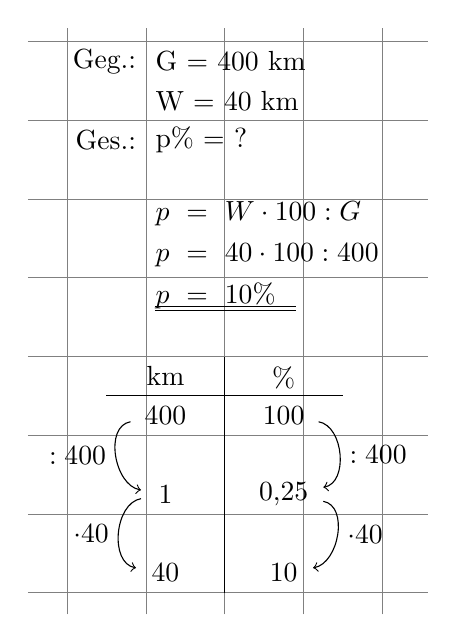
\begin{tikzpicture}[show background grid]
\node[left] at (0,-0.25) {Geg.: };
\node[right] at (0,-0.25) {G = 400 km};
\node[right] at (0,-0.75) {W = 40 km};
\node[left] at (0,-1.25) {Ges.: };
\node[right] at (0,-1.25) {p\%  = ? };
\node[below right] at (0,-1.85) {
$\begin{aligned}
p\ &=\ W\cdot 100 : G \\
p\ &=\ 40\cdot 100 : 400\ \\
\makebox[0pt][l]{\uuline{\phantom{p\%\ =\ 10\% }}}
p\ &=\ 10\% 
\end{aligned}$};

\draw[black] (1cm,-4cm) -- (1cm,-7cm); 
\draw[black] (-0.5 cm,-4.5cm) -- (2.5cm,-4.5cm); 
\node[below] at (0.25 cm,-4cm) {km};
\node[below] at  (1.75 cm,-4cm) {\%};
\node[circle] (1) at (0.25 cm,-4.75cm) {400};
\node[circle] (2) at (0.25 cm,-5.75cm) {1};
\node[circle] (3) at (0.25 cm,-6.75cm) {40};
\node[circle] (4) at (1.75 cm,-4.75cm) {100};
\node[circle] (5) at (1.75 cm,-5.75cm) {0,25};
\node[circle] (6) at (1.75 cm,-6.75cm) {10};
\draw[->] (1) to [out=190,in=170] node[left] {$:400$}  (2) ;
\draw[->] (2) to [out=190,in=170] node[left] {$\cdot 40$}  (3) ;
\draw[->] (4) to [out=350,in=10] node[right] {$:400$}  (5) ;
\draw[->] (5) to [out=350,in=10] node[right] {$\cdot40$}  (6) ;
\end{tikzpicture}
\endgroup
&
j)&
\begingroup\setlength{\jot}{0.02cm}
\tikzstyle{background grid}=[draw, black!15,step=.5cm]
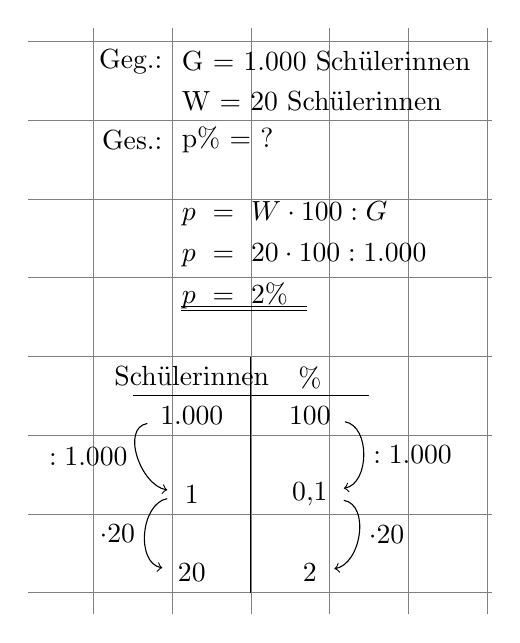
\begin{tikzpicture}[show background grid]
\node[left] at (0,-0.25) {Geg.: };
\node[right] at (0,-0.25) {G = 1.000 Schülerinnen};
\node[right] at (0,-0.75) {W = 20 Schülerinnen};
\node[left] at (0,-1.25) {Ges.: };
\node[right] at (0,-1.25) {p\%  = ? };
\node[below right] at (0,-1.85) {
$\begin{aligned}
p\ &=\ W\cdot 100 : G \\
p\ &=\ 20\cdot 100 : 1.000\ \\
\makebox[0pt][l]{\uuline{\phantom{p\%\ =\ 2\% }}}
p\ &=\ 2\% 
\end{aligned}$};

\draw[black] (1cm,-4cm) -- (1cm,-7cm); 
\draw[black] (-0.5 cm,-4.5cm) -- (2.5cm,-4.5cm); 
\node[below] at (0.25 cm,-4cm) {Schülerinnen};
\node[below] at  (1.75 cm,-4cm) {\%};
\node[circle] (1) at (0.25 cm,-4.75cm) {1.000};
\node[circle] (2) at (0.25 cm,-5.75cm) {1};
\node[circle] (3) at (0.25 cm,-6.75cm) {20};
\node[circle] (4) at (1.75 cm,-4.75cm) {100};
\node[circle] (5) at (1.75 cm,-5.75cm) {0,1};
\node[circle] (6) at (1.75 cm,-6.75cm) {2};
\draw[->] (1) to [out=190,in=170] node[left] {$:1.000$}  (2) ;
\draw[->] (2) to [out=190,in=170] node[left] {$\cdot 20$}  (3) ;
\draw[->] (4) to [out=350,in=10] node[right] {$:1.000$}  (5) ;
\draw[->] (5) to [out=350,in=10] node[right] {$\cdot20$}  (6) ;
\end{tikzpicture}
\endgroup
\\\hline
k)&
\begingroup\setlength{\jot}{0.02cm}
\tikzstyle{background grid}=[draw, black!15,step=.5cm]
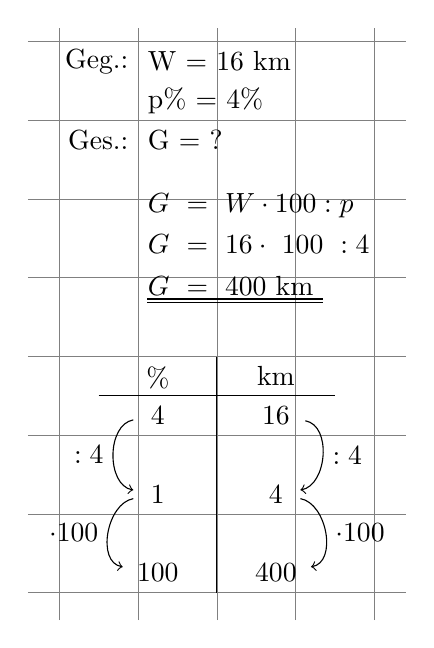
\begin{tikzpicture}[show background grid]
\node[left] at (0,-0.25) {Geg.: };
\node[right] at (0,-0.25) {W = 16 km};
\node[right] at (0,-0.75) {p\% = 4\%};
\node[left] at (0,-1.-0.25) {Ges.: };
\node[right] at (0,-1.-0.25) {G  = ? };
\node[below right] at (0,-1.75) {
$\begin{aligned}
G\ &=\ W\cdot 100 : p \\
G\ &=\ 16\cdot\ 100\ :4 \\
\makebox[0pt][l]{\uuline{\phantom{G\%\ =\ 400\ \mbox{km}}}}
G\ &=\ 400\ \mbox{km}
\end{aligned}$};

\draw[black] (1cm,-4cm) -- (1cm,-7cm); 
\draw[black] (-0.5 cm,-4.5cm) -- (2.5cm,-4.5cm); 
\node[below] at (0.25 cm,-4cm) {\%};
\node[below] at  (1.75 cm,-4cm) {km};
\node[circle] (1) at (0.25 cm,-4.75cm) {4};
\node[circle] (2) at (0.25 cm,-5.75cm) {1};
\node[circle] (3) at (0.25 cm,-6.75cm) {100};
\node[circle] (4) at (1.75 cm,-4.75cm) {16};
\node[circle] (5) at (1.75 cm,-5.75cm) {4};
\node[circle] (6) at (1.75 cm,-6.75cm) {400};
\draw[->] (1) to [out=190,in=170] node[left] {$:4$}  (2) ;
\draw[->] (2) to [out=190,in=170] node[left] {$\cdot 100$}  (3) ;
\draw[->] (4) to [out=350,in=10] node[right] {$:4$}  (5) ;
\draw[->] (5) to [out=350,in=10] node[right] {$\cdot100$}  (6) ;
\end{tikzpicture}
\endgroup
&
l)&
\begingroup\setlength{\jot}{0.02cm}
\tikzstyle{background grid}=[draw, black!15,step=.5cm]
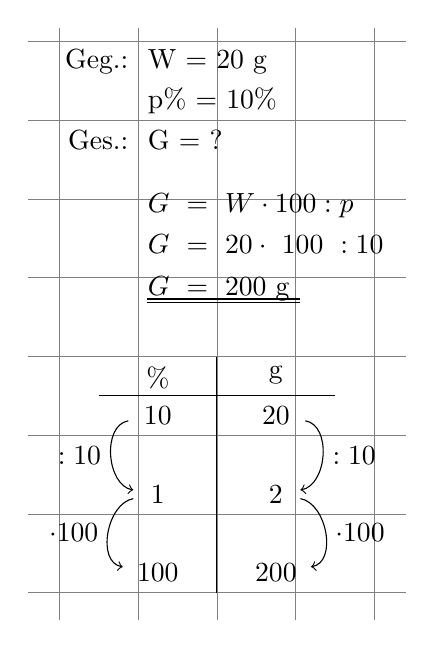
\begin{tikzpicture}[show background grid]
\node[left] at (0,-0.25) {Geg.: };
\node[right] at (0,-0.25) {W = 20 g};
\node[right] at (0,-0.75) {p\% = 10\%};
\node[left] at (0,-1.-0.25) {Ges.: };
\node[right] at (0,-1.-0.25) {G  = ? };
\node[below right] at (0,-1.75) {
$\begin{aligned}
G\ &=\ W\cdot 100 : p \\
G\ &=\ 20\cdot\ 100\ :10 \\
\makebox[0pt][l]{\uuline{\phantom{G\%\ =\ 200\ \mbox{g}}}}
G\ &=\ 200\ \mbox{g}
\end{aligned}$};

\draw[black] (1cm,-4cm) -- (1cm,-7cm); 
\draw[black] (-0.5 cm,-4.5cm) -- (2.5cm,-4.5cm); 
\node[below] at (0.25 cm,-4cm) {\%};
\node[below] at  (1.75 cm,-4cm) {g};
\node[circle] (1) at (0.25 cm,-4.75cm) {10};
\node[circle] (2) at (0.25 cm,-5.75cm) {1};
\node[circle] (3) at (0.25 cm,-6.75cm) {100};
\node[circle] (4) at (1.75 cm,-4.75cm) {20};
\node[circle] (5) at (1.75 cm,-5.75cm) {2};
\node[circle] (6) at (1.75 cm,-6.75cm) {200};
\draw[->] (1) to [out=190,in=170] node[left] {$:10$}  (2) ;
\draw[->] (2) to [out=190,in=170] node[left] {$\cdot 100$}  (3) ;
\draw[->] (4) to [out=350,in=10] node[right] {$:10$}  (5) ;
\draw[->] (5) to [out=350,in=10] node[right] {$\cdot100$}  (6) ;
\end{tikzpicture}
\endgroup
\\\hline
m)&
\begingroup\setlength{\jot}{0.02cm}
\tikzstyle{background grid}=[draw, black!15,step=.5cm]
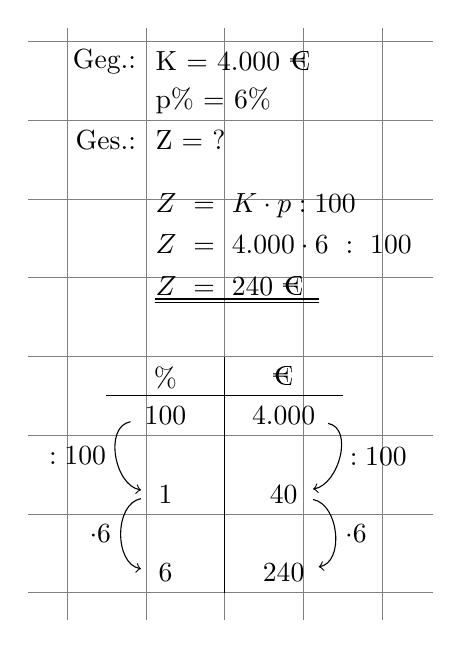
\begin{tikzpicture}[show background grid]
\node[left] at (0,-0.25) {Geg.: };
\node[right] at (0,-0.25) {K = 4.000 €};
\node[right] at (0,-0.75) {p\% = 6\%};
\node[left] at (0,-1.-0.25) {Ges.: };
\node[right] at (0,-1.-0.25) {Z  = ? };
\node[below right] at (0,-1.75) {
$\begin{aligned}
Z\ &=\ K\cdot p : 100 \\
Z\ &=\ 4.000\cdot 6\ :\ 100 \\
\makebox[0pt][l]{\uuline{\phantom{W\%\ =\ 240\ \mbox{€}}}}
Z\ &=\ 240\ \mbox{€}
\end{aligned}$};

\draw[black] (1cm,-4cm) -- (1cm,-7cm); 
\draw[black] (-0.5 cm,-4.5cm) -- (2.5cm,-4.5cm); 
\node[below] at (0.25 cm,-4cm) {\%};
\node[below] at  (1.75 cm,-4cm) {€};
\node[circle] (1) at (0.25 cm,-4.75cm) {100};
\node[circle] (2) at (0.25 cm,-5.75cm) {1};
\node[circle] (3) at (0.25 cm,-6.75cm) {6};
\node[circle] (4) at (1.75 cm,-4.75cm) {4.000};
\node[circle] (5) at (1.75 cm,-5.75cm) {40};
\node[circle] (6) at (1.75 cm,-6.75cm) {240};
\draw[->] (1) to [out=190,in=170] node[left] {$:100$}  (2) ;
\draw[->] (2) to [out=190,in=170] node[left] {$\cdot 6$}  (3) ;
\draw[->] (4) to [out=350,in=10] node[right] {$:100$}  (5) ;
\draw[->] (5) to [out=350,in=10] node[right] {$\cdot6$}  (6) ;
\end{tikzpicture}
\endgroup
&
n)&
\begingroup\setlength{\jot}{0.02cm}
\tikzstyle{background grid}=[draw, black!15,step=.5cm]
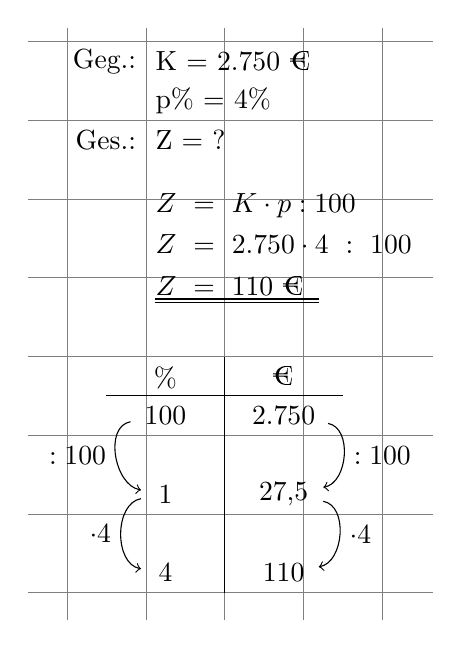
\begin{tikzpicture}[show background grid]
\node[left] at (0,-0.25) {Geg.: };
\node[right] at (0,-0.25) {K = 2.750 €};
\node[right] at (0,-0.75) {p\% = 4\%};
\node[left] at (0,-1.-0.25) {Ges.: };
\node[right] at (0,-1.-0.25) {Z  = ? };
\node[below right] at (0,-1.75) {
$\begin{aligned}
Z\ &=\ K\cdot p : 100 \\
Z\ &=\ 2.750\cdot 4\ :\ 100 \\
\makebox[0pt][l]{\uuline{\phantom{W\%\ =\ 110\ \mbox{€}}}}
Z\ &=\ 110\ \mbox{€}
\end{aligned}$};

\draw[black] (1cm,-4cm) -- (1cm,-7cm); 
\draw[black] (-0.5 cm,-4.5cm) -- (2.5cm,-4.5cm); 
\node[below] at (0.25 cm,-4cm) {\%};
\node[below] at  (1.75 cm,-4cm) {€};
\node[circle] (1) at (0.25 cm,-4.75cm) {100};
\node[circle] (2) at (0.25 cm,-5.75cm) {1};
\node[circle] (3) at (0.25 cm,-6.75cm) {4};
\node[circle] (4) at (1.75 cm,-4.75cm) {2.750};
\node[circle] (5) at (1.75 cm,-5.75cm) {27,5};
\node[circle] (6) at (1.75 cm,-6.75cm) {110};
\draw[->] (1) to [out=190,in=170] node[left] {$:100$}  (2) ;
\draw[->] (2) to [out=190,in=170] node[left] {$\cdot 4$}  (3) ;
\draw[->] (4) to [out=350,in=10] node[right] {$:100$}  (5) ;
\draw[->] (5) to [out=350,in=10] node[right] {$\cdot4$}  (6) ;
\end{tikzpicture}
\endgroup
\\\hline
o)&
\begingroup\setlength{\jot}{0.02cm}
\tikzstyle{background grid}=[draw, black!15,step=.5cm]
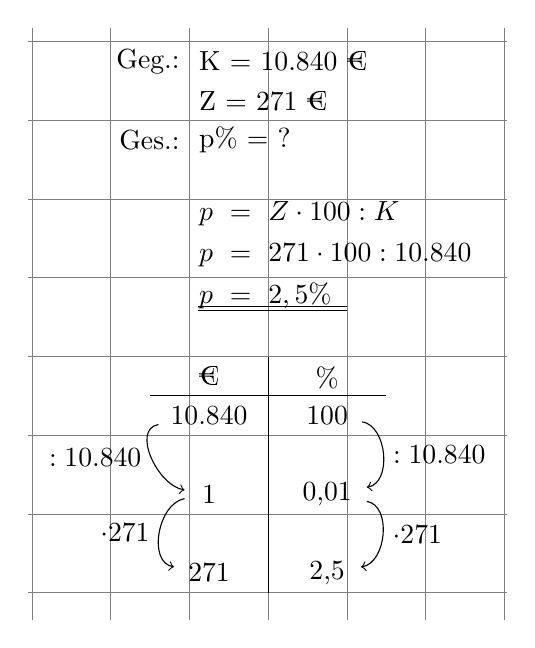
\begin{tikzpicture}[show background grid]
\node[left] at (0,-0.25) {Geg.: };
\node[right] at (0,-0.25) {K = 10.840 €};
\node[right] at (0,-0.75) {Z = 271 €};
\node[left] at (0,-1.25) {Ges.: };
\node[right] at (0,-1.25) {p\%  = ? };
\node[below right] at (0,-1.85) {
$\begin{aligned}
p\ &=\ Z\cdot 100 : K \\
p\ &=\ 271\cdot 100 : 10.840\ \\
\makebox[0pt][l]{\uuline{\phantom{p\%\ =\ 2,5\% }}}
p\ &=\ 2,5\% 
\end{aligned}$};

\draw[black] (1cm,-4cm) -- (1cm,-7cm); 
\draw[black] (-0.5 cm,-4.5cm) -- (2.5cm,-4.5cm); 
\node[below] at (0.25 cm,-4cm) {€};
\node[below] at  (1.75 cm,-4cm) {\%};
\node[circle] (1) at (0.25 cm,-4.75cm) {10.840};
\node[circle] (2) at (0.25 cm,-5.75cm) {1};
\node[circle] (3) at (0.25 cm,-6.75cm) {271};
\node[circle] (4) at (1.75 cm,-4.75cm) {100};
\node[circle] (5) at (1.75 cm,-5.75cm) {0,01};
\node[circle] (6) at (1.75 cm,-6.75cm) {2,5};
\draw[->] (1) to [out=190,in=170] node[left] {$:10.840$}  (2) ;
\draw[->] (2) to [out=190,in=170] node[left] {$\cdot 271$}  (3) ;
\draw[->] (4) to [out=350,in=10] node[right] {$:10.840$}  (5) ;
\draw[->] (5) to [out=350,in=10] node[right] {$\cdot271$}  (6) ;
\end{tikzpicture}
\endgroup
&
p)&
\begingroup\setlength{\jot}{0.02cm}
\tikzstyle{background grid}=[draw, black!15,step=.5cm]
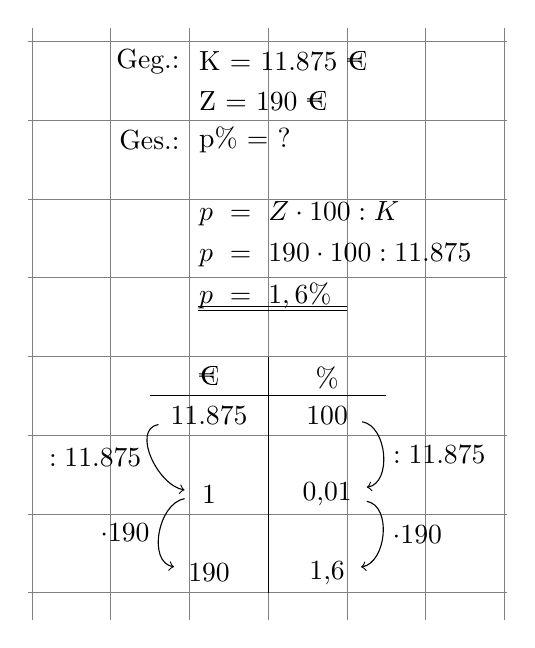
\begin{tikzpicture}[show background grid]
\node[left] at (0,-0.25) {Geg.: };
\node[right] at (0,-0.25) {K = 11.875 €};
\node[right] at (0,-0.75) {Z = 190 €};
\node[left] at (0,-1.25) {Ges.: };
\node[right] at (0,-1.25) {p\%  = ? };
\node[below right] at (0,-1.85) {
$\begin{aligned}
p\ &=\ Z\cdot 100 : K \\
p\ &=\ 190\cdot 100 : 11.875\ \\
\makebox[0pt][l]{\uuline{\phantom{p\%\ =\ 1,6\% }}}
p\ &=\ 1,6\% 
\end{aligned}$};

\draw[black] (1cm,-4cm) -- (1cm,-7cm); 
\draw[black] (-0.5 cm,-4.5cm) -- (2.5cm,-4.5cm); 
\node[below] at (0.25 cm,-4cm) {€};
\node[below] at  (1.75 cm,-4cm) {\%};
\node[circle] (1) at (0.25 cm,-4.75cm) {11.875};
\node[circle] (2) at (0.25 cm,-5.75cm) {1};
\node[circle] (3) at (0.25 cm,-6.75cm) {190};
\node[circle] (4) at (1.75 cm,-4.75cm) {100};
\node[circle] (5) at (1.75 cm,-5.75cm) {0,01};
\node[circle] (6) at (1.75 cm,-6.75cm) {1,6};
\draw[->] (1) to [out=190,in=170] node[left] {$:11.875$}  (2) ;
\draw[->] (2) to [out=190,in=170] node[left] {$\cdot 190$}  (3) ;
\draw[->] (4) to [out=350,in=10] node[right] {$:11.875$}  (5) ;
\draw[->] (5) to [out=350,in=10] node[right] {$\cdot190$}  (6) ;
\end{tikzpicture}
\endgroup
\\\hline
q)&
\begingroup\setlength{\jot}{0.02cm}
\tikzstyle{background grid}=[draw, black!15,step=.5cm]
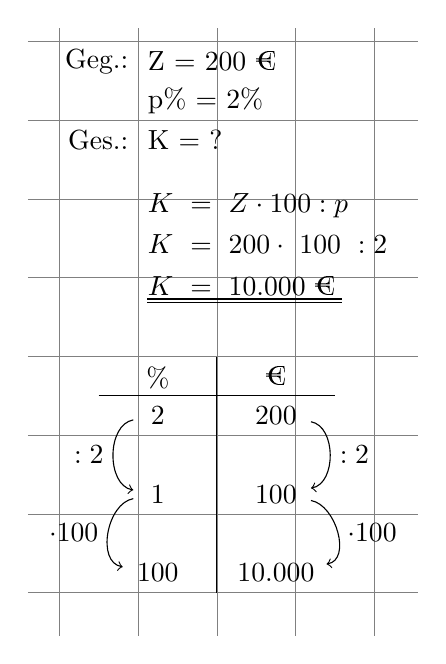
\begin{tikzpicture}[show background grid]
\node[left] at (0,-0.25) {Geg.: };
\node[right] at (0,-0.25) {Z = 200 €};
\node[right] at (0,-0.75) {p\% = 2\%};
\node[left] at (0,-1.-0.25) {Ges.: };
\node[right] at (0,-1.-0.25) {K  = ? };
\node[below right] at (0,-1.75) {
$\begin{aligned}
K\ &=\ Z\cdot 100 : p \\
K\ &=\ 200\cdot\ 100\ :2 \\
\makebox[0pt][l]{\uuline{\phantom{G\%\ =\ 10.000\ \mbox{€}}}}
K\ &=\ 10.000\ \mbox{€}
\end{aligned}$};

\draw[black] (1cm,-4cm) -- (1cm,-7cm); 
\draw[black] (-0.5 cm,-4.5cm) -- (2.5cm,-4.5cm); 
\node[below] at (0.25 cm,-4cm) {\%};
\node[below] at  (1.75 cm,-4cm) {€};
\node[circle] (1) at (0.25 cm,-4.75cm) {2};
\node[circle] (2) at (0.25 cm,-5.75cm) {1};
\node[circle] (3) at (0.25 cm,-6.75cm) {100};
\node[circle] (4) at (1.75 cm,-4.75cm) {200};
\node[circle] (5) at (1.75 cm,-5.75cm) {100};
\node[circle] (6) at (1.75 cm,-6.75cm) {10.000};
\draw[->] (1) to [out=190,in=170] node[left] {$:2$}  (2) ;
\draw[->] (2) to [out=190,in=170] node[left] {$\cdot 100$}  (3) ;
\draw[->] (4) to [out=350,in=10] node[right] {$:2$}  (5) ;
\draw[->] (5) to [out=350,in=10] node[right] {$\cdot100$}  (6) ;
\end{tikzpicture}
\endgroup
&
r)&
\begingroup\setlength{\jot}{0.02cm}
\tikzstyle{background grid}=[draw, black!15,step=.5cm]
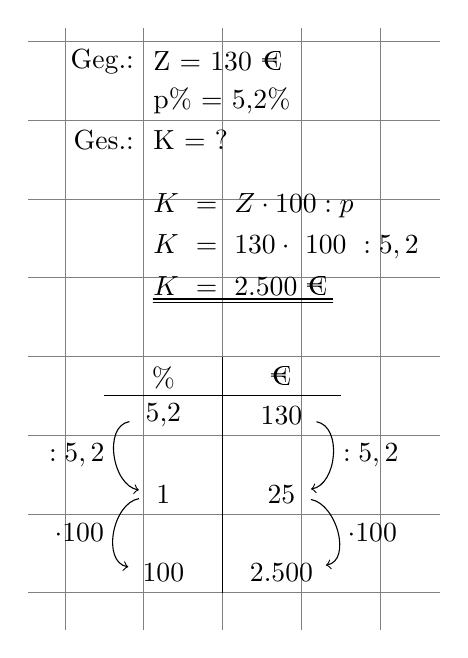
\begin{tikzpicture}[show background grid]
\node[left] at (0,-0.25) {Geg.: };
\node[right] at (0,-0.25) {Z = 130 €};
\node[right] at (0,-0.75) {p\% = 5,2\%};
\node[left] at (0,-1.-0.25) {Ges.: };
\node[right] at (0,-1.-0.25) {K  = ? };
\node[below right] at (0,-1.75) {
$\begin{aligned}
K\ &=\ Z\cdot 100 : p \\
K\ &=\ 130\cdot\ 100\ :5,2 \\
\makebox[0pt][l]{\uuline{\phantom{G\%\ =\ 2.500\ \mbox{€}}}}
K\ &=\ 2.500\ \mbox{€}
\end{aligned}$};

\draw[black] (1cm,-4cm) -- (1cm,-7cm); 
\draw[black] (-0.5 cm,-4.5cm) -- (2.5cm,-4.5cm); 
\node[below] at (0.25 cm,-4cm) {\%};
\node[below] at  (1.75 cm,-4cm) {€};
\node[circle] (1) at (0.25 cm,-4.75cm) {5,2};
\node[circle] (2) at (0.25 cm,-5.75cm) {1};
\node[circle] (3) at (0.25 cm,-6.75cm) {100};
\node[circle] (4) at (1.75 cm,-4.75cm) {130};
\node[circle] (5) at (1.75 cm,-5.75cm) {25};
\node[circle] (6) at (1.75 cm,-6.75cm) {2.500};
\draw[->] (1) to [out=190,in=170] node[left] {$:5,2$}  (2) ;
\draw[->] (2) to [out=190,in=170] node[left] {$\cdot 100$}  (3) ;
\draw[->] (4) to [out=350,in=10] node[right] {$:5,2$}  (5) ;
\draw[->] (5) to [out=350,in=10] node[right] {$\cdot100$}  (6) ;
\end{tikzpicture}
\endgroup
\\\hline
s)&
\begingroup\setlength{\jot}{0.02cm}
\tikzstyle{background grid}=[draw, black!15,step=.5cm]
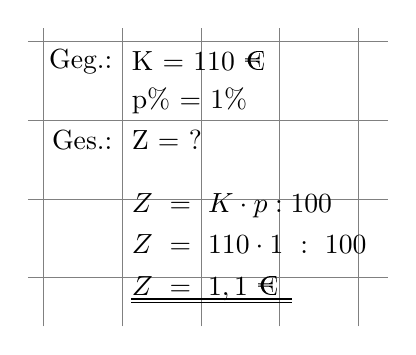
\begin{tikzpicture}[show background grid]
\node[left] at (0,-0.25) {Geg.: };
\node[right] at (0,-0.25) {K = 110 €};
\node[right] at (0,-0.75) {p\% = 1\%};
\node[left] at (0,-1.-0.25) {Ges.: };
\node[right] at (0,-1.-0.25) {Z  = ? };
\node[below right] at (0,-1.75) {
$\begin{aligned}
Z\ &=\ K\cdot p : 100 \\
Z\ &=\ 110\cdot 1\ :\ 100 \\
\makebox[0pt][l]{\uuline{\phantom{W\%\ =\ 1,1\ \mbox{€}}}}
Z\ &=\ 1,1\ \mbox{€}
\end{aligned}$};
\end{tikzpicture}
\endgroup
&
t)&
\begingroup\setlength{\jot}{0.02cm}
\tikzstyle{background grid}=[draw, black!15,step=.5cm]
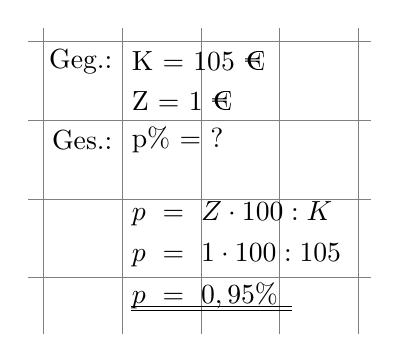
\begin{tikzpicture}[show background grid]
\node[left] at (0,-0.25) {Geg.: };
\node[right] at (0,-0.25) {K = 105 €};
\node[right] at (0,-0.75) {Z = 1 €};
\node[left] at (0,-1.25) {Ges.: };
\node[right] at (0,-1.25) {p\%  = ? };
\node[below right] at (0,-1.85) {
$\begin{aligned}
p\ &=\ Z\cdot 100 : K \\
p\ &=\ 1\cdot 100 : 105\ \\
\makebox[0pt][l]{\uuline{\phantom{p\%\ =\ 0,95\% }}}
p\ &=\ 0,95\% 
\end{aligned}$};
\end{tikzpicture}
\endgroup
\\\hline
u)&
\begingroup\setlength{\jot}{0.15cm}
\tikzstyle{background grid}=[draw, black!15,step=.5cm]
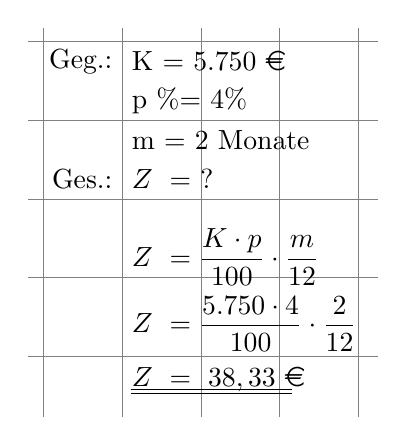
\begin{tikzpicture}[show background grid]
\node[left] at (0,-0.25) {Geg.: };
\node[right] at (0,-0.25) {K\ =\ 5.750\ \euro{}};
\node[right] at (0,-0.75) {p\ \%=\ 4\%};
\node[right] at (0,-1.25) {m\ =\ 2\ Monate};
\node[left] at (0,-1.75) {Ges.: };
\node[right] at (0,-1.75) {$ Z\ =\ ?$};
\node[below right] at (0,-2.25) {
$\begin{aligned}
Z\ &=\frac{K\cdot p}{100}\cdot \frac{m}{12} \\
Z\ &=\frac{5.750\cdot 4}{100}\cdot \frac{2}{12} \\
\makebox[0pt][l]{\uuline{\phantom{Z\ =\ 38,33\ \euro{} }}}
Z\ &=\ 38,33\ \mbox{\euro{}} 
\end{aligned}$};
\end{tikzpicture}
\endgroup
&
v)&
\begingroup\setlength{\jot}{0.15cm}
\tikzstyle{background grid}=[draw, black!15,step=.5cm]
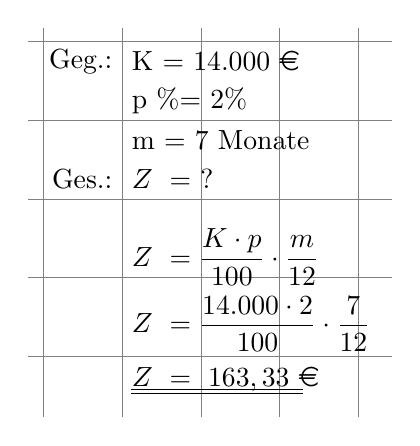
\begin{tikzpicture}[show background grid]
\node[left] at (0,-0.25) {Geg.: };
\node[right] at (0,-0.25) {K\ =\ 14.000\ \euro{}};
\node[right] at (0,-0.75) {p\ \%=\ 2\%};
\node[right] at (0,-1.25) {m\ =\ 7\ Monate};
\node[left] at (0,-1.75) {Ges.: };
\node[right] at (0,-1.75) {$ Z\ =\ ?$};
\node[below right] at (0,-2.25) {
$\begin{aligned}
Z\ &=\frac{K\cdot p}{100}\cdot \frac{m}{12} \\
Z\ &=\frac{14.000\cdot 2}{100}\cdot \frac{7}{12} \\
\makebox[0pt][l]{\uuline{\phantom{Z\ =\ 163,33\ \euro{} }}}
Z\ &=\ 163,33\ \mbox{\euro{}} 
\end{aligned}$};
\end{tikzpicture}
\endgroup
\\\hline
w)&\pbox{5cm}{
Nach 1 Jahren: \\
$\begin{aligned}
Z_1&=K_{start}\cdot p\% \\
&=4.280 € \cdot 0,025 \\
&=107 €\\
K_1&=K_{start}+Z \\
&=4.280 €+ 107 €\\
\makebox[0pt][l]{\uuline{\phantom{$K_1=4.387 €\\$} } }
K_1&=4.387 €\\
\end{aligned}$ \\
Nach 2 Jahren: \\
$\begin{aligned}
Z_2&=K_1\cdot p\% \\
&=4.387 € \cdot 0,025 \\
&=109,67 €\\
K_2&=K_1+Z \\
&=4.387 €+ 109,67 €\\
\makebox[0pt][l]{\uuline{\phantom{$K_2=4.496,68 €\\$} } }
K_2&=4.496,68 €\\
\end{aligned}$ \\
}
&
x)&\pbox{5cm}{
Nach 1 Jahren: \\
$\begin{aligned}
Z_1&=K_{start}\cdot p\% \\
&=13.950 € \cdot 0,02 \\
&=279 €\\
K_1&=K_{start}+Z \\
&=13.950 €+ 279 €\\
\makebox[0pt][l]{\uuline{\phantom{$K_1=14.229 €\\$} } }
K_1&=14.229 €\\
\end{aligned}$ \\
Nach 2 Jahren: \\
$\begin{aligned}
Z_2&=K_1\cdot p\% \\
&=14.229 € \cdot 0,02 \\
&=284,58 €\\
K_2&=K_1+Z \\
&=14.229 €+ 284,58 €\\
\makebox[0pt][l]{\uuline{\phantom{$K_2=14.513,58 €\\$} } }
K_2&=14.513,58 €\\
\end{aligned}$ \\
}
\\\hline
\end{xltabular}
\vspace{0.5cm}
\end{document}